\documentclass[conference]{IEEEtran}
\IEEEoverridecommandlockouts
\usepackage{cite}
\usepackage{amsmath,amssymb,amsfonts}
\usepackage{algorithm}
\usepackage{algorithmic}
\usepackage{graphicx}
\usepackage{booktabs}
\usepackage{array}

\def\BibTeX{{\rm B\kern-.05em{\sc i\kern-.025em b}\kern-.08em
    T\kern-.1667em\lower.7ex\hbox{E}\kern-.125emX}}

\begin{document}

\title{FINDEC: An Agentic Framework for Risk-Aware Financial Decision
Support with Per-Agent Evaluation}

\author{
\IEEEauthorblockN{Mansi, Sudesh Rani, and Kanu Goel}
\IEEEauthorblockA{
Department of Computer Science and Engineering\\
Punjab Engineering College (Deemed to be University)\\
Chandigarh, India\\
\{mansi.bt22cse, sudeshrani, kanugoel\}@pec.edu.in
}
}

\maketitle

\begin{abstract}
Retail investors face fragmented evidence, while agentic financial systems
that could consolidate it are usually judged on portfolio return alone and
almost always forecast price direction. We present FINDEC, an open-source
framework in which a Planner routes a query, a Researcher gathers structured
evidence, an Analyst estimates market uncertainty, and a Risk Manager
converts that uncertainty into a sized recommendation. Departing from
end-to-end return accounting, we evaluate each agent separately. Across 196
equities and ten years, comprising 43{,}512 out-of-sample observations, we
find a pronounced asymmetry in what is estimable: the rank correlation
between forecast and outcome is $-0.074$ for return direction but $+0.554$
for realised volatility and $-0.320$ for forward drawdown. Directional
accuracy at a one-day horizon is $0.4875$, with a confidence interval that
excludes chance from below. The consequence propagates downstream, where a
constant-exposure portfolio matched to the system's own average exposure
attains a higher Sharpe ratio, a shallower drawdown and a larger return than
the sized policy. One mechanism nonetheless survives: withholding a
recommendation when confidence is low raises accuracy monotonically from
$52.1\%$ to $57.5\%$ as coverage falls from $100\%$ to $10\%$. We argue that
uncertainty estimation and selective prediction are firmer foundations for
financial agents than directional forecasting.
\end{abstract}

%% ============================================================
\section{Introduction}
\label{sec:intro}
%% ============================================================
Deciding what to do with a holding draws on four distinct competences:
locating relevant information, reasoning over it, forming a view about what
happens next, and deciding how much capital that view justifies. Institutions
separate these among research analysts, quantitative modellers and risk
officers. Retail investors possess none of that division of labour and must
reconcile conflicting sources unaided.

Agentic artificial intelligence offers the same decomposition in software.
Recent systems assign roles to cooperating agents and coordinate them toward
a trading decision, with FinRobot~\cite{yang2024finrobot},
TradingAgents~\cite{xiao2024tradingagents} and FinGPT~\cite{yang2023fingpt}
representing the direction of travel. Two properties recur across this
literature. First, evaluation is almost exclusively end-to-end: a portfolio
return, a Sharpe ratio, occasionally a drawdown. Second, the quantity being
predicted is nearly always the direction of price movement.

Both properties deserve scrutiny. An aggregate return statistic cannot
localise a failure, so a system that underperforms offers no guidance about
which component to repair. And the choice of prediction target is rarely
justified; direction is adopted because it maps conveniently onto a buy or
sell label, not because evidence establishes it as the most estimable
quantity available.

This paper takes the second question first. Before asking whether an agent
predicts direction well, we ask whether direction is predictable at all from
the information such systems consume, and how it compares against other
targets computable from the same data. We then trace what the answer implies
for a working multi-agent system, and evaluate every agent on its own terms
rather than through a portfolio aggregate.

\subsection{Research Questions}
\textbf{RQ1.} Does task specialisation across cooperating agents improve
financial decision support, and can each agent's contribution be isolated?
\textbf{RQ2.} Which quantities should an Analyst Agent estimate, given what
is empirically predictable from market data?
\textbf{RQ3.} How should estimated uncertainty propagate into a
recommendation, and when should a recommendation be withheld?

\subsection{Contributions}
\begin{itemize}
\item An open-source agentic framework combining planning, evidence
retrieval, uncertainty estimation and risk-aware synthesis, deployable on
commodity CPU hardware.
\item A per-agent evaluation protocol in which the Planner, Researcher,
Analyst and Risk Manager are measured separately against metrics appropriate
to each, rather than through portfolio return alone.
\item A measured predictability asymmetry across candidate targets on 196
equities and ten years, showing that second-moment quantities are
substantially more estimable than direction.
\item Evidence that confidence-aware abstention improves decision quality
where directional forecasting does not, together with a matched-exposure
control that distinguishes genuine risk management from reduced exposure.
\end{itemize}

%% ============================================================
\section{Related Work}
\label{sec:related}
%% ============================================================

\subsection{Multi-Agent Financial AI}
Dividing financial analysis among specialised agents improves modularity and
mirrors institutional practice. TradingAgents~\cite{xiao2024tradingagents}
assigns analysis, research and execution to distinct roles;
FinRobot~\cite{yang2024finrobot} layers large language models over financial
tooling. These systems demonstrate feasibility but depend on commercial model
endpoints, proprietary data or accelerator hardware. FINDEC adopts the
decomposition while keeping the analytical path deterministic and executable
on standard processors, which preserves auditability and reproducibility.

\subsection{Financial Language Models}
Domain-adapted encoders such as FinBERT~\cite{araci2019finbert} improve
sentiment extraction from financial text, and later work refines
domain-specific features and neutral-class handling~\cite{sun2025financial}.
Such models are valuable for live interpretation but complicate retrospective
evaluation, since a pretrained encoder may already encode the period under
test.

\subsection{Volatility Forecasting}
Unlike returns, volatility exhibits pronounced persistence, and models
exploiting it are long established. The heterogeneous autoregressive
specification of Corsi regresses future realised variance on daily, weekly
and monthly components and remains a standard reference point; generalised
autoregressive conditional heteroskedasticity models and exponentially
weighted schemes provide the other conventional baselines. Patton showed that
when the volatility target is observed only through a noisy proxy, many loss
functions rank forecasts incorrectly, and identified squared error and QLIKE
as robust choices. We adopt QLIKE for that reason.

\subsection{Risk-Aware Recommendation}
Risk estimation traditionally rests on realised volatility, Value at Risk and
its conditional variant. Recent frameworks pair statistical estimates with
linguistic signals to detect regime change and emphasise uncertainty
quantification over return maximisation~\cite{chen2026smart}, while
agent-based portfolio systems integrate sentiment with optimisation under
shifting conditions~\cite{mantshimuli2026toward}. Evaluation practice has
received less attention than modelling; Sullivan and colleagues established
that apparent profitability shrinks once the search producing it is priced
in, a concern that transfers directly to comparisons among agent
architectures. The Risk Manager described here is deliberately transparent,
mapping estimated uncertainty and a stated tolerance onto a position size
without solving a portfolio optimisation.

%% ============================================================
\section{FINDEC Architecture}
\label{sec:arch}
%% ============================================================

\begin{figure}[htbp]
\centering
\includegraphics[width=\linewidth]{FINDEC-Arch1.png}
\caption{FINDEC architecture. A Planner routes each query to the agents its
intent requires; the Researcher and Analyst run concurrently; the Risk
Manager consumes their estimates rather than directional votes. Dashed
arrows denote outbound calls whose failure surfaces as an explicit
availability flag.}
\label{fig:arch}
\end{figure}

FINDEC is organised as three deployment tiers and four cooperating agents.
The presentation tier is a Next.js application; a Node.js service handles
authentication, routing and report persistence; and analysis runs in a Python
service exposing the agent pipeline. Figure~\ref{fig:arch} shows the
arrangement.

What distinguishes the agentic organisation from a fixed pipeline is that the
set of agents invoked is decided per query rather than hard-coded. The
Planner converts a free-text request into a structured task graph naming the
intent, the securities involved, the decision horizon, and the subtasks
required. The orchestrator dispatches exactly those subtasks and no others. A
request for a definition dispatches nothing; a request bearing on the user's
own capital always dispatches the Risk Manager, whether or not the user asked
about downside.

Two mechanisms support this. Each agent returns a typed result carrying its
own confidence, the timestamp of the newest datum it consulted, and the
window it drew from, so a decision can be reconstructed exactly and any
information postdating it detected. Second, an agent unable to reach its
source returns an explicit unavailable status rather than a neutral value, so
the synthesis stage reweights over what remains instead of treating an
absence as evidence.

%% ============================================================
\section{Agent Design}
\label{sec:agents}
%% ============================================================

\begin{figure}[htbp]
\centering
\includegraphics[width=\linewidth]{FINDEC_agents.png}
\caption{Signals exchanged between agents. The Analyst emits a distribution
and a calibrated confidence rather than a directional label.}
\label{fig:agents}
\end{figure}

\subsection{Planner Agent}
The Planner classifies a query into one of eleven intents and emits a
schema-validated task graph. The intent vocabulary is derived from observed
usage rather than invented: published analysis of retail questions put to a
financial assistant finds that interpretation and screening dominate, while
explicit requests for advice form a small minority. The Planner resolves
company names to exchange symbols, relative horizons to day counts, and
infers risk posture from how a user describes loss tolerance rather than from
an explicit label alone.

Two post-conditions are enforced after classification rather than requested
of the model, since a prompt expresses an intention while a post-condition
enforces one. Queries classified as definitional dispatch no agents. Queries
placing the user's capital at risk always attach a downside estimate.

\subsection{Researcher Agent}
The Researcher assembles structured evidence rather than prose. Retrieved
articles are filtered for financial relevance, deduplicated by source, and
scored by a transformer encoder, with a lexicon scorer retained as a
fallback. Each article carries a recency weight with a three-day half-life,
and the agent returns an aggregate polarity, an agreement-based confidence,
and the citations backing them.

Its scope requires a statement. Historical news at the access tier used here
extends approximately thirty days into the past, so the Researcher cannot
participate in a decade-long retrospective evaluation; requests beyond that
window are refused by the provider. Even with an archive, scoring historical
headlines with a pretrained encoder would introduce a subtler difficulty,
since the encoder's parameters may already encode the period under test. The
Researcher is therefore evaluated prospectively, on live operation, and
excluded from the retrospective results of Section~\ref{sec:evaluation}.

\subsection{Analyst Agent}
\label{sec:analyst}
The Analyst is the component this paper examines most closely, because
everything downstream conditions on what it produces.

\subsubsection{Why direction is the wrong target}
The original Analyst emitted a directional label from an ensemble of ridge
regression and logistic classification over engineered features. Evaluating
that design at scale rather than on a handful of names produced the result in
Section~\ref{sec:analyst-eval}: the rank correlation between predicted and
realised direction is negative at every horizon tested. A point estimate of
an unforecastable quantity is not a useful object, and every mechanism that
scales exposure by such an estimate scales it by noise.

\subsubsection{Feature construction}
Features are computed from a strictly backward-looking window. Beyond
conventional technical terms, the set emphasises quantities relevant to
dispersion rather than direction: realised volatility over multiple scales,
the ratio between short- and long-horizon volatility, downside semivariance,
rolling skewness and kurtosis, drawdown depth and time since peak, volume
relative to its own trend, and return relative to a market proxy. All are
standardised using statistics drawn from the training window alone.

\subsubsection{Estimating a distribution}
The redesigned Analyst emits a distribution rather than a label. Its
governing principle follows from the measured asymmetry: estimate the second
moment, remain honest about the first, and derive the remainder. For horizon
$h$, dispersion is estimated from realised variance, while the central
estimate is shrunk toward zero and capped at a small fraction of the
estimated standard deviation:
\begin{equation}
\hat{\sigma}_h = \sqrt{h}\,\hat{\sigma}_{\text{daily}}, \qquad
|\hat{\mu}_h| \leq \kappa\,\hat{\sigma}_h,
\label{eq:dist}
\end{equation}
with $\kappa = 0.25$. The asymmetry is deliberate. Asserting a mean produced
a negative information coefficient; estimating dispersion honestly leaves the
output useful regardless, because sizing keys on the ratio
$\hat{\mu}_h/\hat{\sigma}_h$ rather than on the level of either term.

Given $\hat{\sigma}_h$, further quantities follow analytically rather than
from separately fitted models. The probability of appreciation is
$\Phi(\hat{\mu}_h/\hat{\sigma}_h)$. The probability that the path falls a
fraction $x$ below its starting value within the horizon follows from the
reflection principle,
\begin{equation}
P(\text{drawdown} > x) = 2\,\Phi\!\left(\frac{-x}{\hat{\sigma}_h}\right),
\label{eq:dd}
\end{equation}
and expected maximum drawdown scales with $\hat{\sigma}_h$. Deriving these
rather than fitting them separately guarantees mutual consistency and
concentrates estimation risk in one place, where it can be measured.

\subsubsection{Confidence and abstention}
A raw confidence is formed from $|\hat{\mu}_h/\hat{\sigma}_h|$ and mapped
through a reliability curve fitted on realised outcomes, so a stated value
corresponds to an observed frequency rather than to model self-report. When
the ratio falls below a threshold the Analyst abstains, returning no view
rather than a weak one. Abstention is a first-class output: given the
evidence in Section~\ref{sec:analyst-eval}, no view is frequently the correct
answer, and a system unable to express it will manufacture one.

\subsubsection{Cross-sectional rank}
Because ranking a security against its peers is a different problem from
forecasting its absolute movement, the Analyst also reports a percentile rank
of $\hat{\mu}_h/\hat{\sigma}_h$ within the day's universe. This requires a
universe-level call and cannot be produced by per-ticker invocation.

\subsection{Risk Manager Agent}
The Risk Manager consumes estimates, not votes. Position scale follows from
the volatility estimate against a risk budget; the drawdown probability of
Eq.~\eqref{eq:dd} acts as a constraint rather than a score, capping exposure
when it exceeds the profile's tolerance; and calibrated confidence modulates
size within that budget. An abstaining Analyst suppresses the recommendation
entirely, which the interface distinguishes from a hold. Profiles cap
exposure at $6\%$, $10\%$ and $16\%$ of capital.

Position changes take effect on the session after the one whose closing data
produced them. Applying a decision to the same session's return would allow
information in that closing price to influence a position notionally taken
beforehand.

%% ============================================================
\section{Experimental Evaluation}
\label{sec:evaluation}
%% ============================================================

\subsection{Setup}
Results are computed on daily data for 196 US equities spanning ten years,
with at least two constituents per sector. Models refit on a trailing window
and are scored only on subsequent unseen observations. Accuracy figures carry
$95\%$ Wilson intervals. The universe was selected at the end of the sample,
so every constituent survived the period; this survivorship flatters all
reported columns and applies equally to the system and its baselines.

\subsection{Agent-Level Evaluation}
Table~\ref{tab:agents} summarises each agent against a metric appropriate to
its output rather than against portfolio return. Reporting them separately is
what allows a failure to be localised.

\begin{table}[!ht]
\centering
\setlength{\belowcaptionskip}{3pt}
\caption{Agent-level evaluation. Each agent is scored on its own output.}
\vspace{-2.5mm}
\begin{tabular}{
  >{\arraybackslash}m{42pt}
  >{\arraybackslash}m{72pt}
  >{\centering\arraybackslash}m{40pt}
  >{\centering\arraybackslash}m{38pt}
  }
  \toprule
  \textbf{Agent} & \textbf{Metric} & \textbf{Result} & \textbf{Baseline} \\
  \midrule
  Planner    & Intent accuracy      & 0.692 & 0.75 \\
  Researcher & Retrospective coverage & n/a & --- \\
  Analyst    & Rank corr., direction & $-0.074$ & 0 \\
  Analyst    & Rank corr., volatility & $+0.554$ & 0 \\
  Analyst    & Accuracy at $10\%$ coverage & 0.575 & 0.50 \\
  Risk Mgr.  & Sharpe vs matched exposure & 0.381 & 0.539 \\
  \bottomrule
\end{tabular}
\label{tab:agents}
\end{table}

The Planner trails a supervised classifier trained on the source corpus, and
we report it as a component measurement rather than as a contribution. The
Researcher is not scored retrospectively for the reason given in
Section~\ref{sec:agents}. The Analyst rows are developed below; the Risk
Manager row is developed in Section~\ref{sec:sizing}.

\subsection{Analyst Evaluation}
\label{sec:analyst-eval}
Table~\ref{tab:analyst} reports, for each candidate target, the rank
correlation between a forecast built from trailing information and the
realised outcome, plotted in Figure~\ref{fig:results}(a), together with the deployed Analyst's directional accuracy
at three horizons.

\begin{table}[!ht]
\centering
\setlength{\belowcaptionskip}{3pt}
\caption{Analyst evaluation. Upper block: predictability of candidate targets
over 43{,}512 out-of-sample observations at a 21-day horizon. Lower block:
deployed directional accuracy over 8{,}814 decisions, with $95\%$ Wilson
intervals.}
\vspace{-2.5mm}
\begin{tabular}{
  >{\arraybackslash}m{86pt}
  >{\centering\arraybackslash}m{46pt}
  >{\centering\arraybackslash}m{58pt}
  }
  \toprule
  \textbf{Target} & \textbf{Rank corr.} & \textbf{$R^2$} \\
  \midrule
  Direction of return      & $-0.0744$ & 0.014 \\
  Magnitude of return      & $+0.2489$ & 0.108 \\
  \textbf{Realised volatility} & $\mathbf{+0.5543}$ & \textbf{0.286} \\
  Forward maximum drawdown & $-0.3199$ & 0.084 \\
  \midrule
  \textbf{Horizon} & \textbf{Accuracy} & \textbf{95\% CI} \\
  \midrule
  1 day   & 0.4875 & [0.4771, 0.4980] \\
  5 days  & 0.5021 & [0.4916, 0.5126] \\
  21 days & 0.5073 & [0.4968, 0.5178] \\
  \bottomrule
\end{tabular}
\label{tab:analyst}
\end{table}

Volatility is roughly seven times more predictable than direction, and the
directional relationship carries the wrong sign. At one day the accuracy
interval lies wholly below $0.50$: the forecast is significantly worse than
chance, not merely uninformative. At longer horizons it is indistinguishable
from chance.

Volatility forecasting was assessed on the same protocol using QLIKE, which
remains valid when the target is observed through a noisy proxy. Over
5{,}700 forecasts the heterogeneous autoregressive model attains $-6.789$
against $-6.725$ for a random walk, confirming genuine persistence; an
exponentially weighted estimator reaches $-6.823$, so the simplest
conditional baseline is not displaced. Volatility ordering is estimated well
even where its level is not, which is what a sizing rule requires. Drawdown
probabilities derived from Eq.~\eqref{eq:dd} improve on the unconditional
base rate only marginally, and their reliability curve slopes downward,
overstating risk where predicted risk is highest.

\subsection{Confidence-Aware Abstention}
Table~\ref{tab:abstain} and Figure~\ref{fig:results}(b) report accuracy as a
function of coverage, where coverage is the proportion of queries on which
the system commits to a view and abstention removes the least confident.

\begin{table}[!ht]
\centering
\setlength{\belowcaptionskip}{3pt}
\caption{Accuracy against coverage under confidence-based abstention.
5{,}700 out-of-sample decisions; $95\%$ Wilson bounds.}
\vspace{-2.5mm}
\begin{tabular}{
  >{\centering\arraybackslash}m{44pt}
  >{\centering\arraybackslash}m{32pt}
  >{\centering\arraybackslash}m{44pt}
  >{\centering\arraybackslash}m{62pt}
  }
  \toprule
  \textbf{Coverage} & \textbf{$n$} & \textbf{Accuracy} & \textbf{95\% CI} \\
  \midrule
  100\% & 5700 & 0.5205 & [0.5075, 0.5335] \\
  75\%  & 4275 & 0.5273 & [0.5123, 0.5422] \\
  50\%  & 2850 & 0.5375 & [0.5192, 0.5558] \\
  25\%  & 1425 & 0.5621 & [0.5362, 0.5877] \\
  \textbf{10\%} & \textbf{570} & \textbf{0.5754} & \textbf{[0.5345, 0.6154]} \\
  \bottomrule
\end{tabular}
\label{tab:abstain}
\end{table}

\begin{figure*}[!t]
\centering
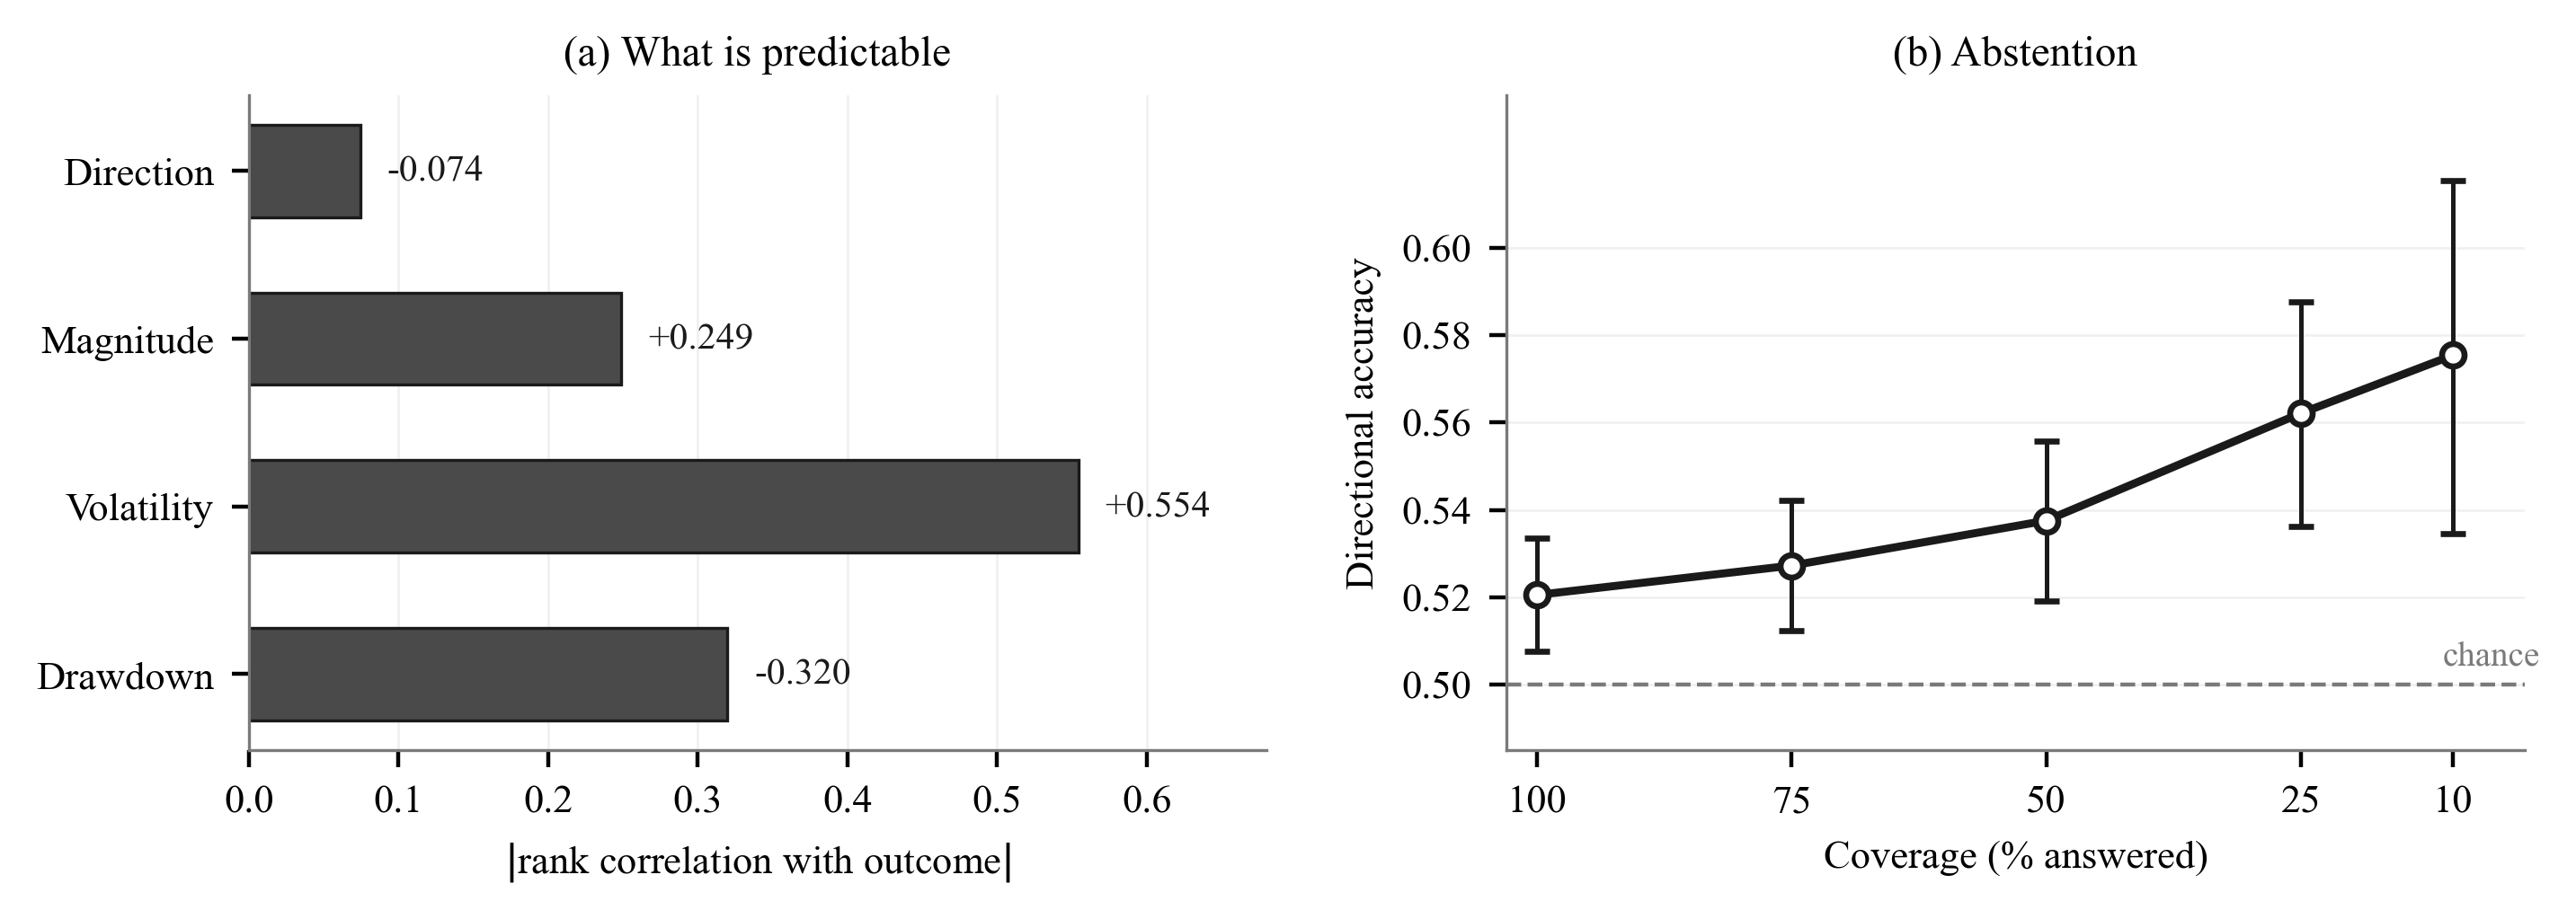
\includegraphics[width=0.92\textwidth]{results_panels.png}
\caption{The two central results. (a) Strength of the relationship between a
forecast built from trailing information and the realised outcome, over
43{,}512 out-of-sample observations at a 21-day horizon; bar length is the
magnitude of the rank correlation and the signed value is annotated. The two
negative signs carry opposite meanings: for direction the forecast is
anti-predictive, whereas for drawdown the negative sign is the expected
relationship, since higher trailing volatility predicts a deeper subsequent
fall. (b) Directional accuracy against coverage under confidence-based
abstention, with $95\%$ Wilson intervals; the dashed line marks chance.}
\label{fig:results}
\end{figure*}

Accuracy rises monotonically as the system answers less often, and every
interval excludes chance. The Analyst cannot forecast direction, yet its
confidence ranks its own reliability.

\subsection{Effect on Position Sizing}
\label{sec:sizing}
Conditioning exposure on an uninformative forecast carries a measurable cost.
We compare the sized policy against a control holding the system's own
average exposure every day with no timing whatsoever, which separates genuine
risk management from simply holding less. The sized policy attains a Sharpe
ratio of $0.381$, an annualised return of $9.97\%$ and a maximum drawdown of
$-38.0\%$; the constant-exposure control at the same average exposure attains
$0.539$, $11.52\%$ and $-33.8\%$, dominating on all three (Figure~\ref{fig:exposure}). A fully invested
arm reproduces buy-and-hold exactly, confirming the harness.

\begin{figure}[!t]
\centering
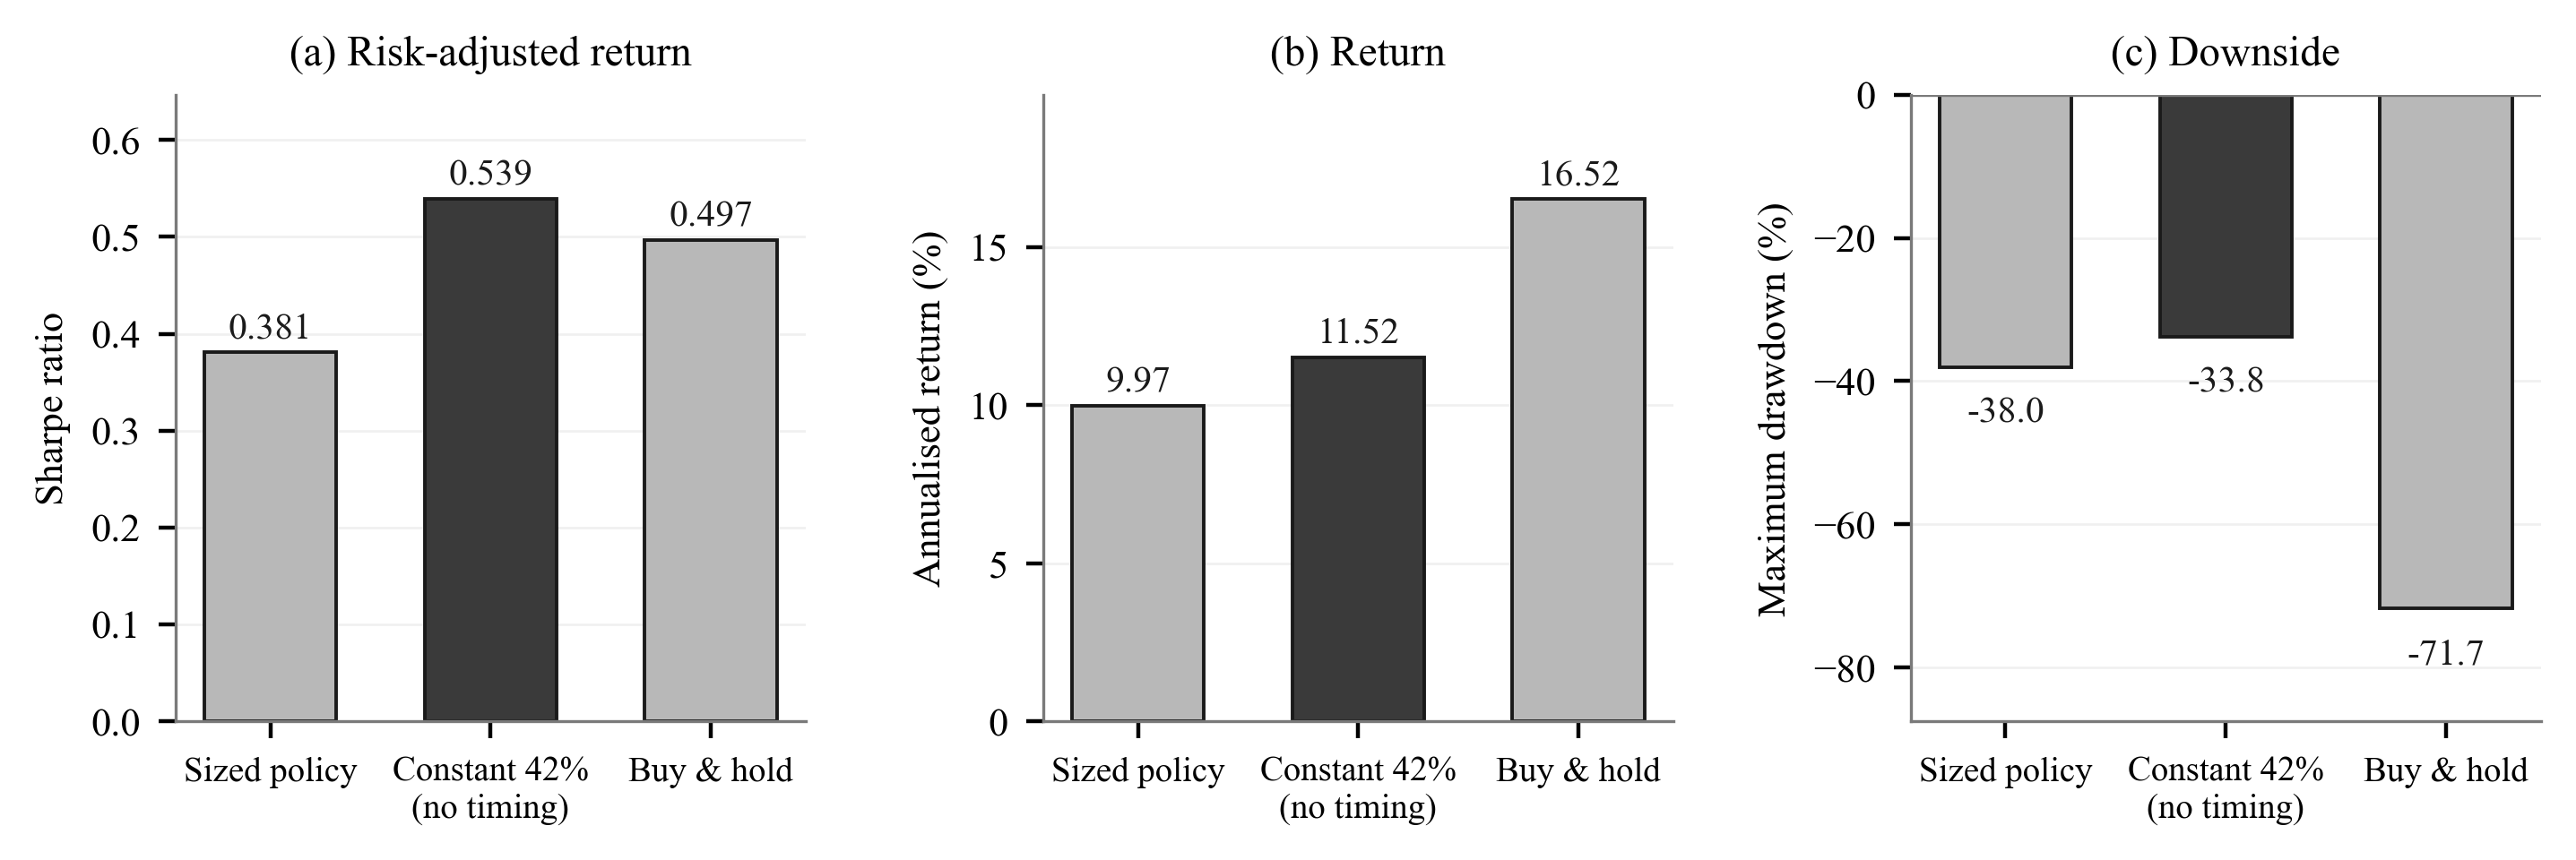
\includegraphics[width=\linewidth]{matched_exposure.png}
\caption{The matched-exposure control. Holding the sized policy's own average
exposure of $42\%$ every day, with no timing whatsoever, beats that policy on
all three measures at once (dark bars). Buy-and-hold earns the most and falls
furthest, which is why comparing against it alone conceals the failure:
reduced exposure lowers drawdown, so any delevered policy resembles risk
management regardless of what its timing contributes.}
\label{fig:exposure}
\end{figure}

Volatility targeting, which requires no directional forecast, was tested
separately across all 196 equities and proved significantly worse than a
constant exposure ($t=-8.80$, $p<0.0001$), prevailing on 47 of 196 names,
though it did reduce drawdown by 3.6 percentage points. Since the Sharpe
ratio is invariant to constant rescaling of exposure, the risk profiles
function as a leverage setting rather than as distinct strategies.

%% ============================================================
\section{Discussion}
\label{sec:discussion}
%% ============================================================

\subsection{Direction remains hard}
Evaluated across 196 equities and a decade, directional forecasting from
technical information is not merely weak but adverse at short horizons. This
is consistent with weak-form efficiency and with the failure of comparable
systems to outperform passive exposure. The implication is not that the
models are poorly tuned; it is that the target is wrong.

The sample size required to settle such claims deserves statement. With a
strategy-to-benchmark correlation near $0.55$, separating a Sharpe
improvement of $+0.30$ at conventional power needs approximately 19{,}692
trading days, whereas the available holdout supports $5.9\%$ power against a
$5\%$ false-positive rate. Breadth does not resolve this, since
contemporaneous equity returns are correlated and 500 names supply roughly
2.85 effective independent units against 2.08 for five. Directional accuracy
and calibration converge within hundreds of observations, which is why they
carry the conclusions here.

\subsection{Uncertainty carries more information}
Volatility and drawdown are substantially more estimable from identical
inputs. The asymmetry is actionable rather than merely descriptive: an
Analyst emitting a distribution supports position sizing, downside
constraints and abstention, none of which require knowing which way a price
will move. Volatility predictability is not profitability, however. A
dependable dispersion estimate improves risk control; it does not by itself
generate return, and the distinction should be preserved in any claim.

An evaluation comparing only against buy-and-hold cannot detect the sizing
failure of Section~\ref{sec:sizing}, because reduced exposure lowers drawdown
and thereby presents as risk management. A matched-exposure control should
accompany any such comparison. The same reasoning applies to execution
timing: applying a decision to the session whose close produced it inflated
mean Sharpe from $0.192$ to $0.724$ in an earlier revision of this system and
reversed its reported outcome, a defect that presented as skill because the
comparison baseline was correctly lagged.

\subsection{Agentic decomposition enables per-agent measurement}
The decomposition's principal benefit here is epistemic. Because the Planner,
Analyst and Risk Manager are separable, a failure can be localised to the
Analyst's target rather than attributed vaguely to the system. An
architecture whose agents emit calibrated estimates with explicit abstention
can be audited component by component; one whose agents emit buy or sell
labels cannot, since a label carries no claim that can be checked against
frequency.

%% ============================================================
\section{Conclusion}
\label{sec:conclusion}
%% ============================================================
FINDEC organises financial decision support into planning, evidence
retrieval, uncertainty estimation and risk-aware synthesis, and evaluates
each agent separately rather than through portfolio return. Measured across
196 equities and ten years, the direction of price movement proves
anti-predictive while realised volatility and forward drawdown are estimated
substantially better from identical inputs. Confidence-aware abstention
raises accuracy from $52.1\%$ to $57.5\%$ as coverage narrows, every interval
excluding chance, and a matched-exposure control shows that reduced exposure
should not be mistaken for risk management. Future work will extend the
Analyst with range-based volatility estimators, obtain archival news
permitting retrospective evaluation of the Researcher, and report the live
prospective deployment now accumulating sealed predictions.

\bibliographystyle{IEEEtran}
\bibliography{references}

\end{document}
